% !TeX root = ../main.tex
% Add the above to each chapter to make compiling the PDF easier in some editors.

\chapter{Related Work}\label{chapter:related_work}

Early work primarily optimized for \ac{FLOP}s, but it is now well understood that minimizing \ac{FLOP}s alone can lead to prohibitively large intermediate tensors and thus excessive memory consumption~\cite{pednault2017pareto}. Therefore, a new set of algorithms have been developed to reduce this effect of the memory. This section reviews these contributions, with a focus on techniques that explicitly reduce memory footprint or data movement.


\section{Treewidth-Based and Graph-Theoretic Methods}

Markov and Shi~\cite{markov2008simulating} established a foundational connection between tensor network contraction and graph theory, showing that the complexity of contraction is governed by the treewidth of the underlying graph. Minimizing treewidth implicitly controls the size of intermediate tensors and therefore peak memory usage. This is due to the treewidth bounding the size of the largest intermediate tensor produced during contraction. A contraction with treewidth $k$ guarantees that no intermediate tensor will have more than $k$ indices. This directly translates to memory savings. Moreover, low treewidth enables efficient dynamic programming algorithms that can compute the optimal contraction sequence in time exponential only in treewidth, not in the total number of tensors.

However, exact treewidth minimization is NP-hard~\cite{dumitrescu2018benchmarking}, motivating heuristic approaches. Subsequent work has leveraged graph partitioning and elimination ordering heuristics to approximate optimal contraction paths. For example, tools such as \texttt{quickbb}~\cite{gogate2012complete} and \texttt{flow-cutter}~\cite{hamann2018graph} have been adapted to tensor contraction problems. These approaches reduce peak memory by limiting separator sizes, though they are not explicitly designed for memory movement.

\section{Hypergraph Partitioning Approaches}

More recent work models tensor networks as hypergraphs, enabling more accurate representation of multi-index tensors. Gray and Kourtis~\cite{gray2021hyper} introduced a hypergraph-based contraction path optimizer that uses partitioning techniques to minimize both \ac{FLOP}s and intermediate tensor sizes. This framework allows explicit incorporation of memory constraints and has been widely adopted in tools such as \texttt{cotengra}.

Hypergraph partitioning methods can be extended to multi-objective optimization, balancing \ac{FLOP}s and memory. For instance, multi-criteria cost functions penalize large intermediate tensors, effectively reducing peak memory usage. However, these methods typically focus on static path selection and do not account for runtime memory movement.

\section{Slicing Techniques}

Slicing is one of the most widely used methods for reducing peak memory. It involves fixing certain indices to specific values, thereby decomposing a large contraction into multiple smaller subproblems. Each slice can be computed independently, significantly reducing memory requirements at the cost of increased total computation. Figure~\ref{fig:index_slicing} illustrates this process.

\begin{figure}[ht]
    \centering
    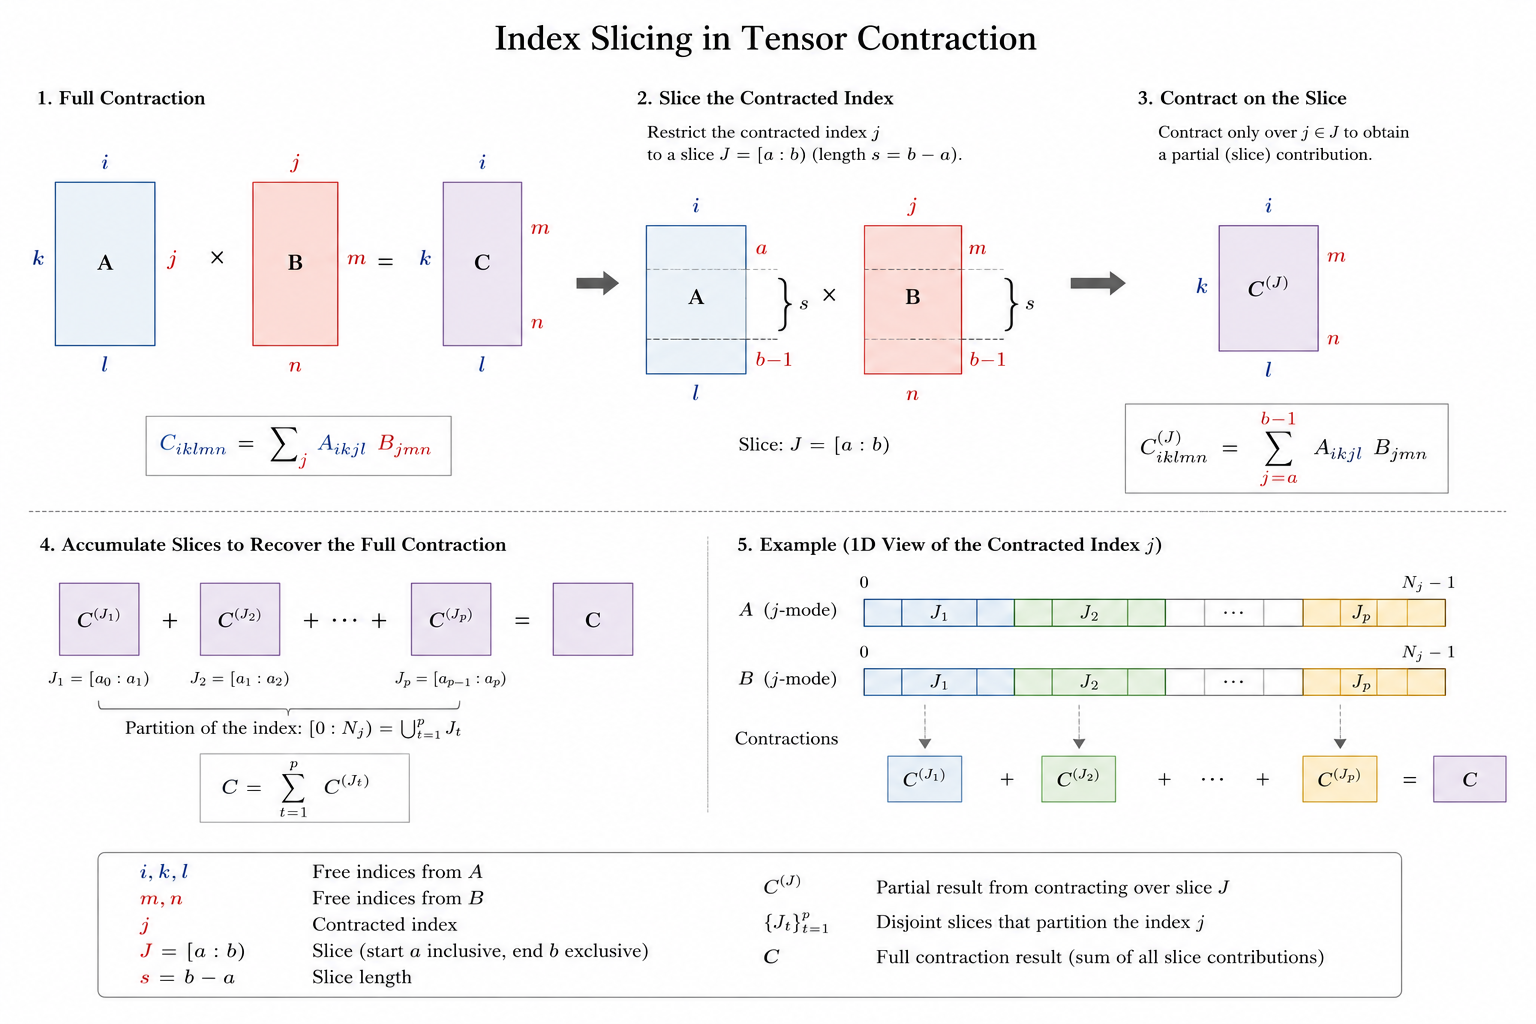
\includegraphics[width=1.325\textwidth,angle=-90]{figures/index_slicing.png}
    \caption{Illustration of index slicing in tensor contraction}
    \label{fig:index_slicing}
\end{figure}

This approach has been extensively used in quantum circuit simulation, including in Google's quantum supremacy experiments~\cite{arute2019quantum}. Later work formalized slicing as an optimization problem, selecting indices to slice in order to trade off memory and runtime~\cite{gray2021hyper}. In practice, slicing is especially attractive when the memory footprint of the original contraction exceeds available RAM, because it can reduce the size of intermediates by several orders of magnitude.

However, slicing also introduces a trade-off between memory and execution cost that must be carefully managed. In the context of quantum circuit simulation, Google's quantum advantage experiment used slicing to reduce the peak memory of a 53-qubit simulation, at the expense of decomposing the contraction into $2^8 = 256$ independent cut instances (paths) for 12 cycles, which exponentially scales to $2^{19} = 524,288$ cut instances for 14 cycles which is more than the unsliced contraction~\cite{arute2019quantum}. 

The benefits of slicing are not limited to raw memory reduction. Because individual slices are independent, they expose a high degree of parallelism and can be distributed across processors or compute nodes with minimal synchronization. This property is especially advantageous for out-of-core or distributed execution, where fitting a single slice into local memory or cache can substantially improve throughput. Several works~\cite{gray2021hyper,huang2021efficient,liu2021sunway,schutski2020simple} therefore treat slicing as a practical mechanism to scale tensor contraction to larger circuits or networks than would otherwise fit on a single device.

While slicing is a powerful technique for enabling contractions that would otherwise be infeasible due to memory limits, it is most effective when used in combination with path optimization and execution-level strategies. Careful selection of slicing indices and integration with low-level data movement optimization are necessary to realize the potential benefits without incurring prohibitive runtime overhead.

\section{Recompression and Tensor Decomposition}

Another class of methods reduces memory by compressing intermediate tensors. Techniques such as singular value decomposition (SVD) and tensor train (TT) decompositions are used to approximate tensors with lower-rank representations.

For example, methods based on matrix product states (MPS)~\cite{schollwock2011density} and tensor trains~\cite{oseledets2011tensor} dynamically truncate intermediate tensors to control memory growth. These approaches are particularly effective in structured problems with low entanglement, but introduce approximation error and may not generalize to arbitrary tensor networks which are the primary focus of this work.

\section{Memory Movement and Data Locality}

While peak memory has received significant attention, memory movement is increasingly recognized as a critical bottleneck. Modern hardware architectures exhibit large disparities between computation speed and memory bandwidth, making data movement a dominant cost~\cite{ballard2011minimizing}.

Efforts to reduce memory movement include blocking and tiling strategies~\cite{li2019analytical, park2003tiling}, which aim to maximize cache reuse, as well as layout transformations that improve data locality. In the context of tensor contractions, permutation of tensor indices plays a key role in determining memory access patterns.

However, most existing work treats permutations as a secondary concern, focusing primarily on algebraic correctness rather than memory efficiency. This represents a significant gap in the literature.

\section{Summary}

The literature on tensor network contraction reveals two complementary lines of work. One line emphasizes pre-contraction optimization, using graph-theoretic and hypergraph partitioning techniques to choose contraction orders that limit intermediate tensor sizes and reduce peak memory across the execution. The other line emphasizes post-contraction execution, using slicing, recompression, and out-of-core scheduling to cope with cases where available memory is insufficient for a single monolithic contraction. Both approaches have advanced the ability to solve larger networks and higher-dimensional problems, but they also expose an important limitation: the predominant focus has been on peak memory and arithmetic cost, while the costs of data movement, tensor layout, and permutation overhead are still treated as subordinate concerns. This gap is especially salient in modern high-performance contexts, where memory bandwidth and cache locality often dominate actual runtime.